\section{Appendix C: Supplementary Signal-Layer Results}

This appendix collects the supporting material for the investor warning layer.

\subsection{Signal figures by asset}

\begin{figure}[H]
    \centering
    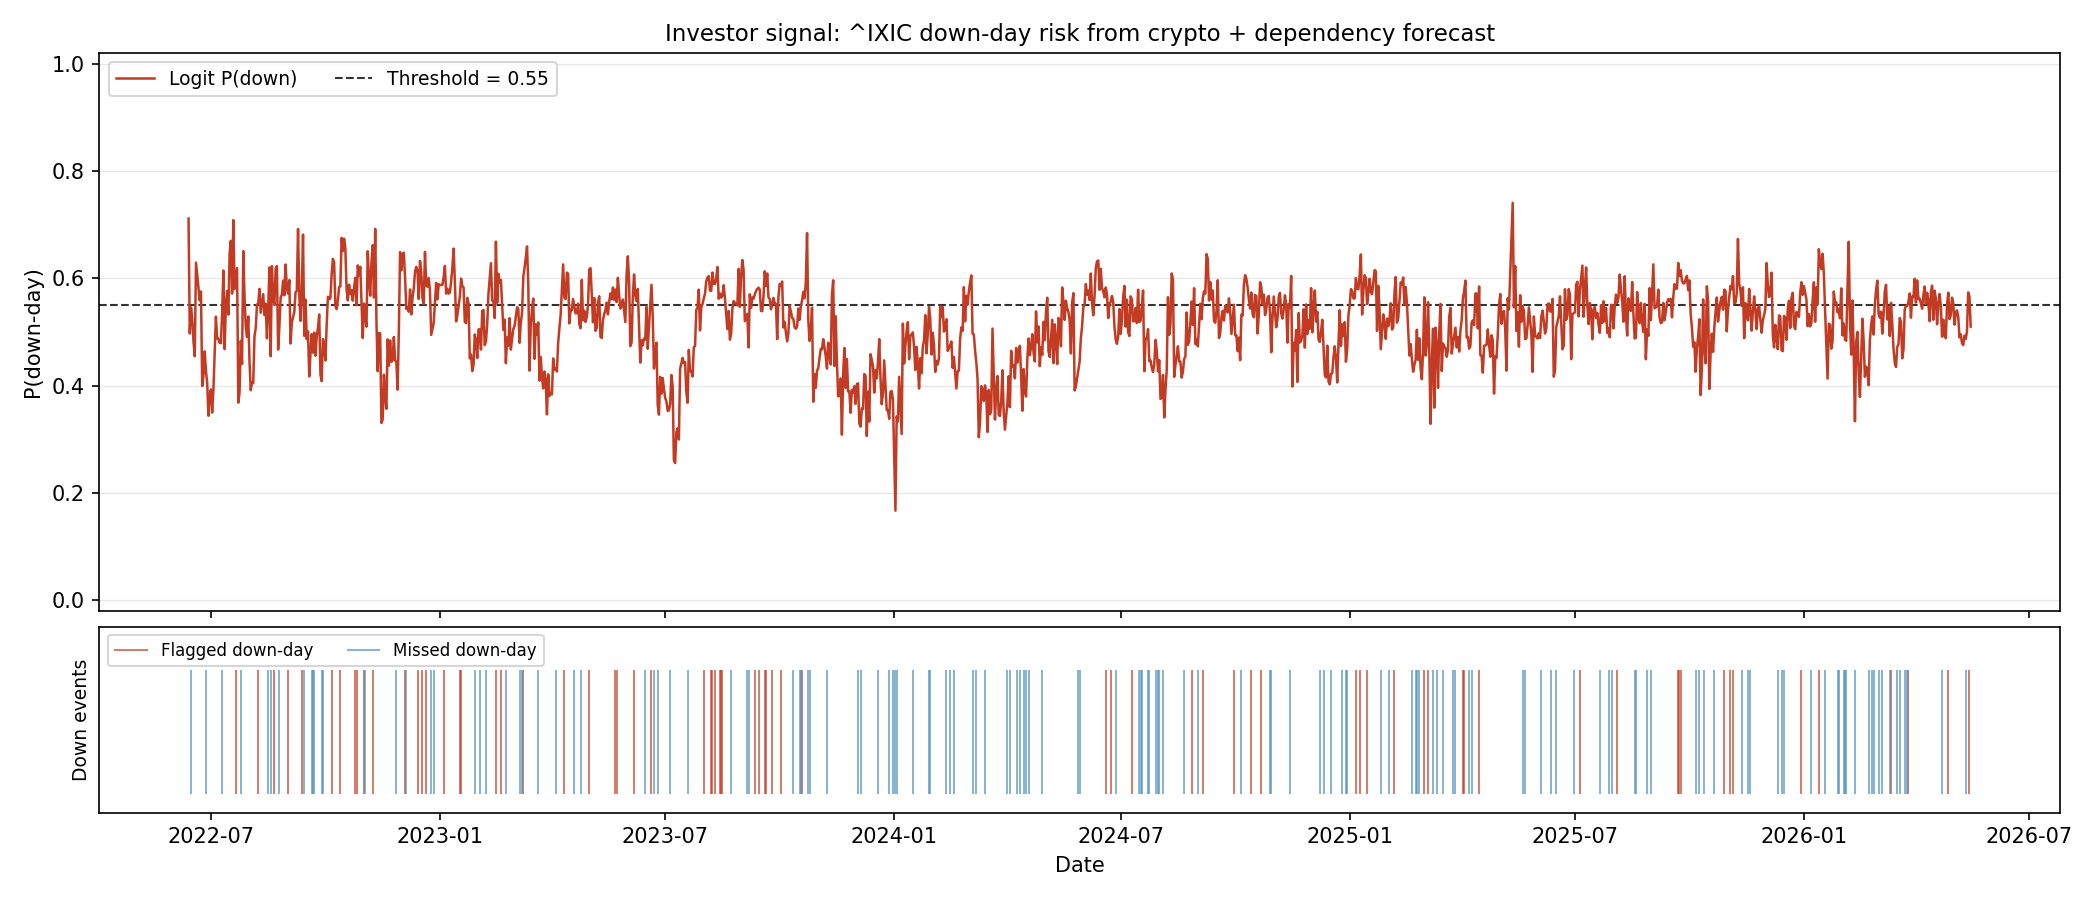
\includegraphics[width=0.9\textwidth]{../outputs/figures/signal_corr_BTC-USD_^IXIC_w30.png}
    \caption{Signal-layer output for the Bitcoin--NASDAQ relation at the 30-day window.}
    \label{fig:app_signal_ixic_w30}
\end{figure}

\begin{figure}[H]
    \centering
    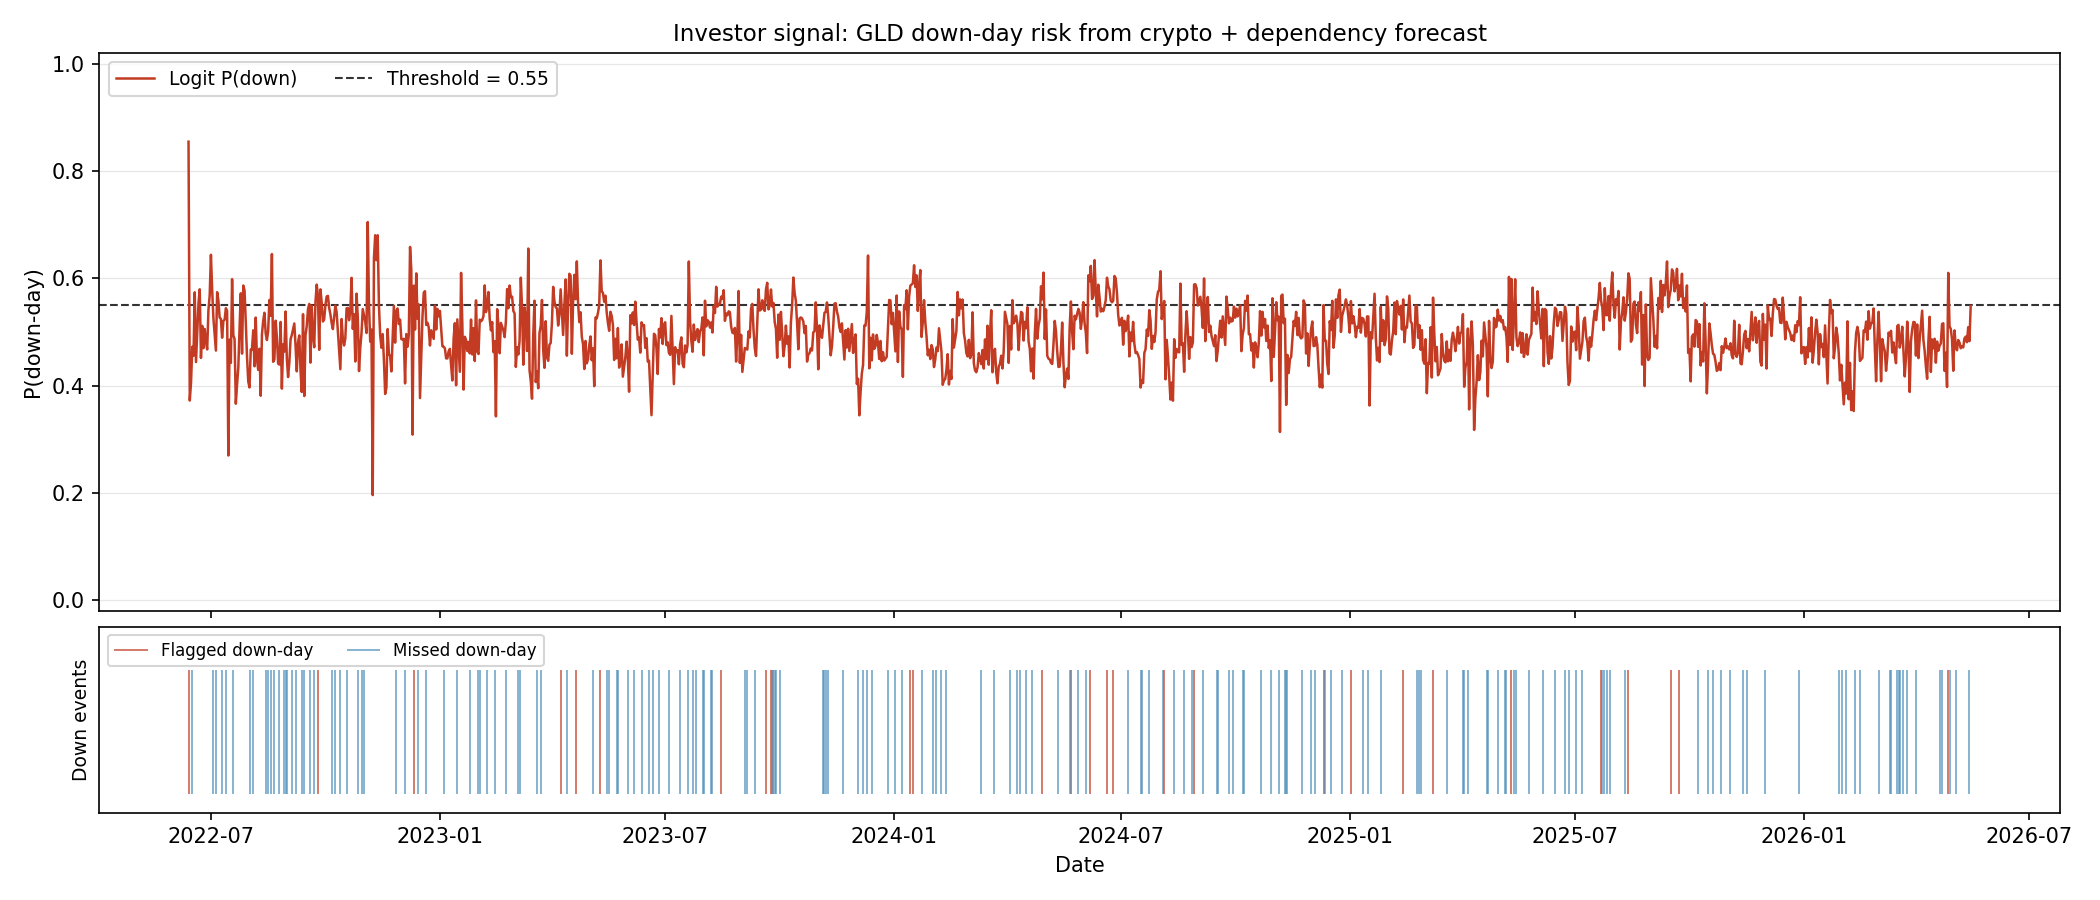
\includegraphics[width=0.9\textwidth]{../outputs/figures/signal_corr_BTC-USD_GLD_w30.png}
    \caption{Signal-layer output for the Bitcoin--gold relation at the 30-day window.}
    \label{fig:app_signal_gld_w30}
\end{figure}

\begin{figure}[H]
    \centering
    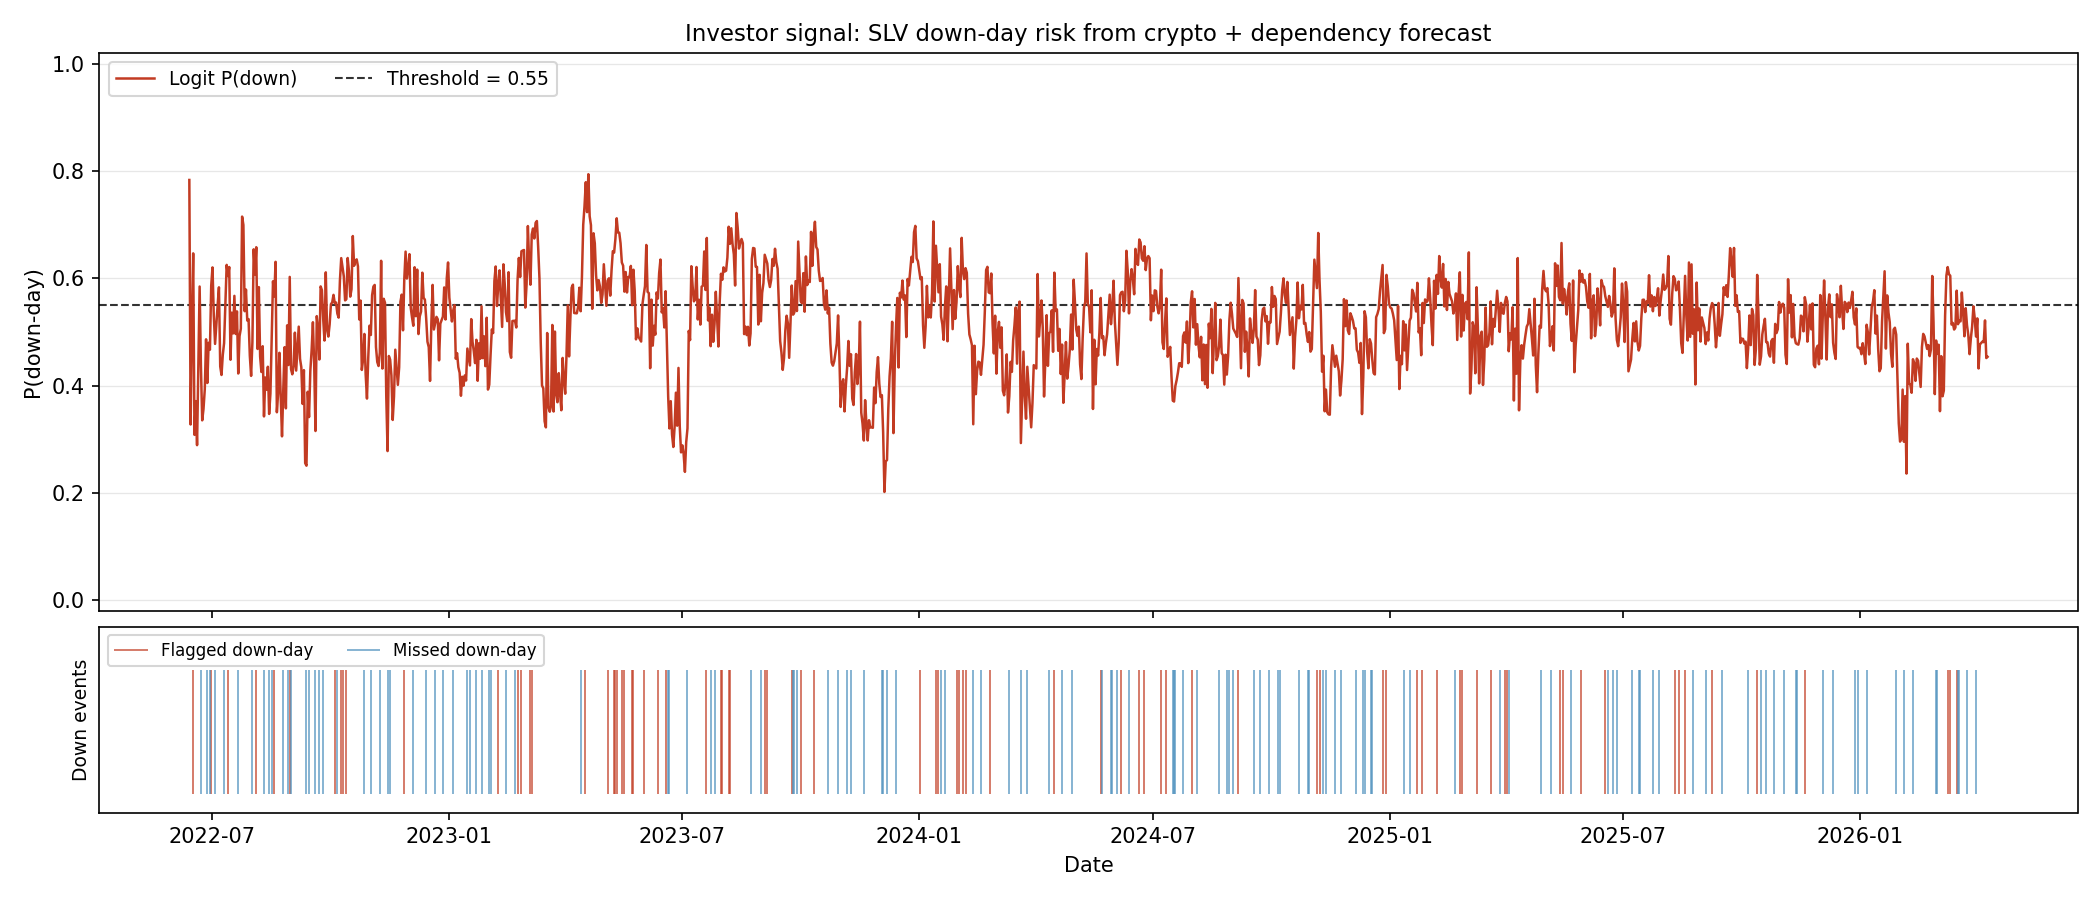
\includegraphics[width=0.9\textwidth]{../outputs/figures/signal_corr_BTC-USD_SLV_w30.png}
    \caption{Signal-layer output for the Bitcoin--silver relation at the 30-day window.}
    \label{fig:app_signal_slv_w30}
\end{figure}

\begin{figure}[H]
    \centering
    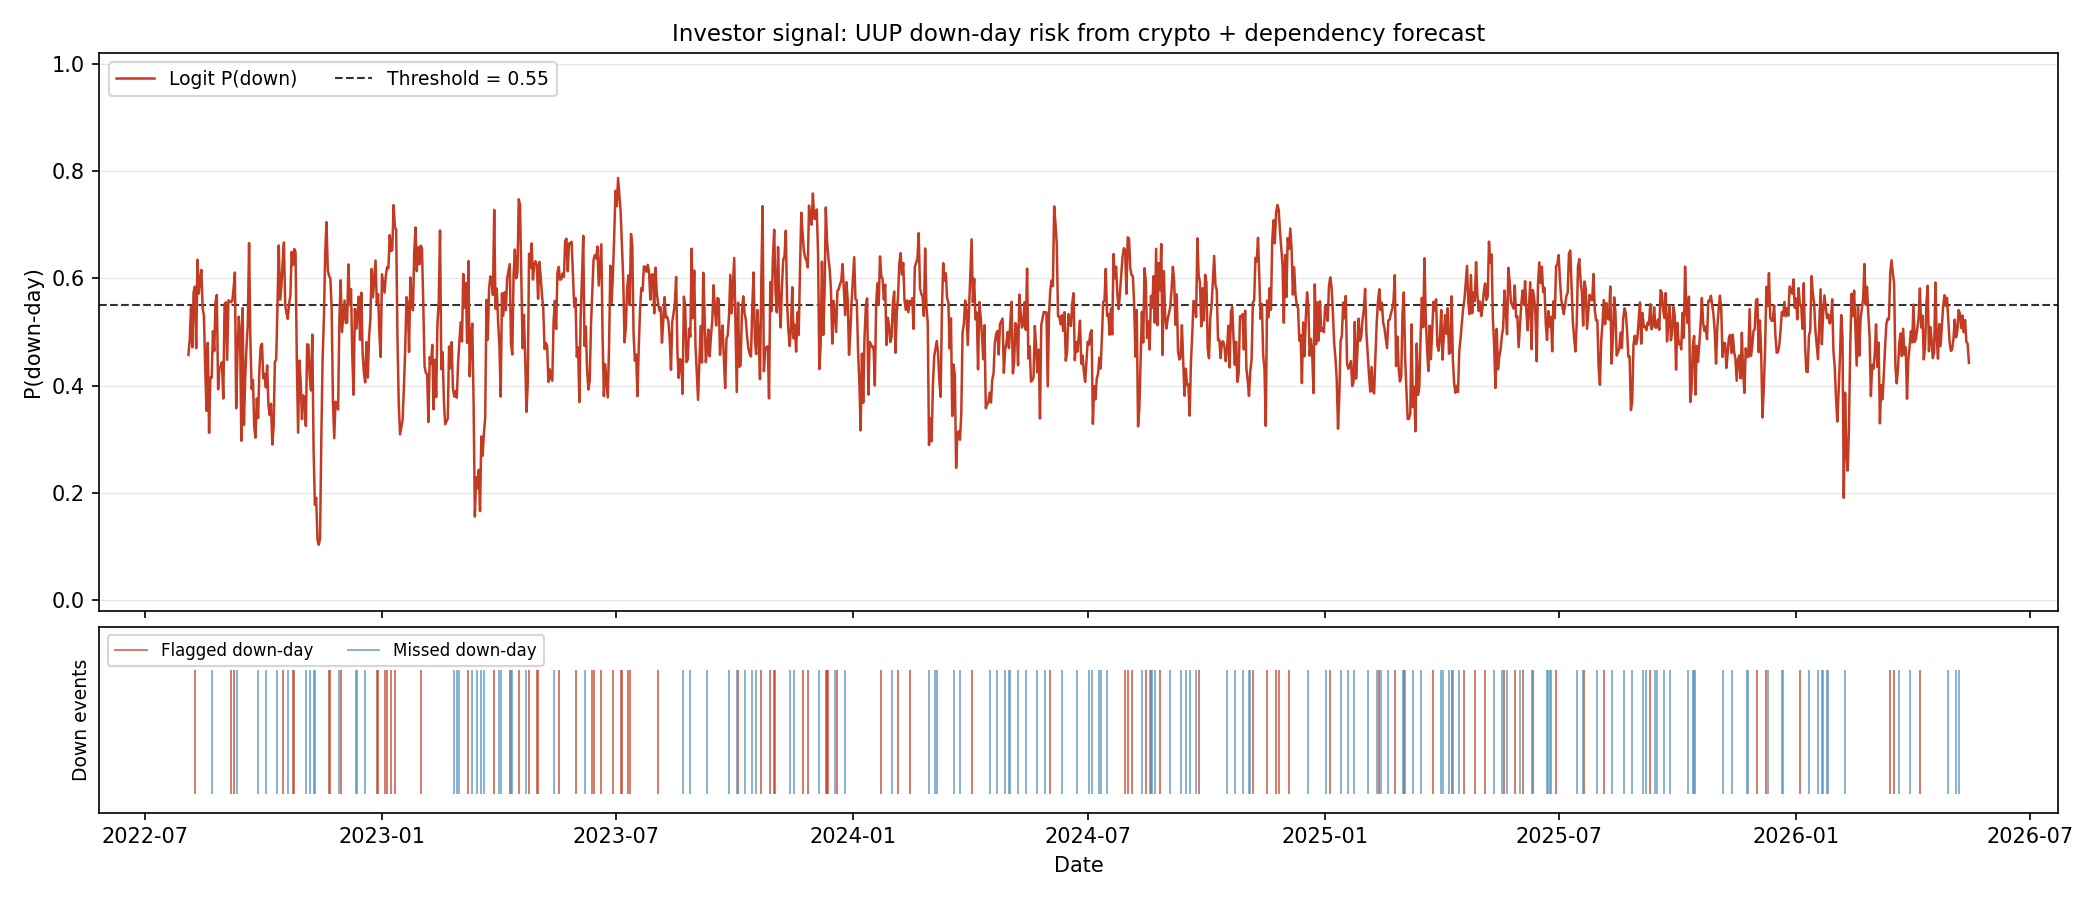
\includegraphics[width=0.9\textwidth]{../outputs/figures/signal_corr_BTC-USD_UUP_w30.png}
    \caption{Signal-layer output for the Bitcoin--UUP relation at the 30-day window.}
    \label{fig:app_signal_uup_w30}
\end{figure}

\subsection{Cross-market warning interpretation}

The signal figures show that the warning layer behaves very differently from market to market. The S\&P~500 produces the clearest warning episodes; NASDAQ is markedly weaker, dipping below chance in several configurations --- probably because its sector concentration adds idiosyncratic noise that the crypto channel cannot see. The metal and dollar targets are noisier but not uniformly useless. The lesson is that the layer should be applied selectively, not across the board.

\subsection{Summary table}

\begin{table}[H]
    \centering
    \caption{Balanced accuracy of the Logit signal layer by asset pair and rolling-window
             length. Family-level averages across all pairs and windows are reported in
             Table~\ref{tab:signal_summary}; this breakdown shows where the signal is
             informative.}
    \label{tab:app_signal_summary}
    \begin{tabular}{lrrrrr}
        \toprule
        Asset pair & $w{=}14$ & $w{=}30$ & $w{=}60$ & $w{=}90$ & Mean \\
        \midrule
        BTC--S\&P 500  & 0.5169 & 0.5308 & 0.5212 & 0.5264 & 0.5238 \\
        BTC--NASDAQ    & 0.5190 & 0.5016 & 0.4865 & 0.4917 & 0.4997 \\
        BTC--Gold      & 0.5053 & 0.5041 & 0.5078 & 0.5202 & 0.5093 \\
        BTC--Silver    & 0.4938 & 0.5187 & 0.5053 & 0.5189 & 0.5092 \\
        BTC--USD index & 0.5071 & 0.5197 & 0.5131 & 0.5204 & 0.5151 \\
        \bottomrule
    \end{tabular}
\end{table}

This breakdown supports the main-text reading. The Bitcoin--S\&P~500 pair is the
strongest and most consistent, peaking at 0.5308 at the 30-day window. Bitcoin--NASDAQ
is the weakest, averaging 0.4997 and falling below the 0.50 chance level at the 60- and
90-day windows. The precious-metal and dollar pairs are positive on average but remain
close to chance. The signal is therefore best applied selectively to broad-equity pairs
rather than uniformly across the asset universe.

\begin{figure}[H]
    \centering
    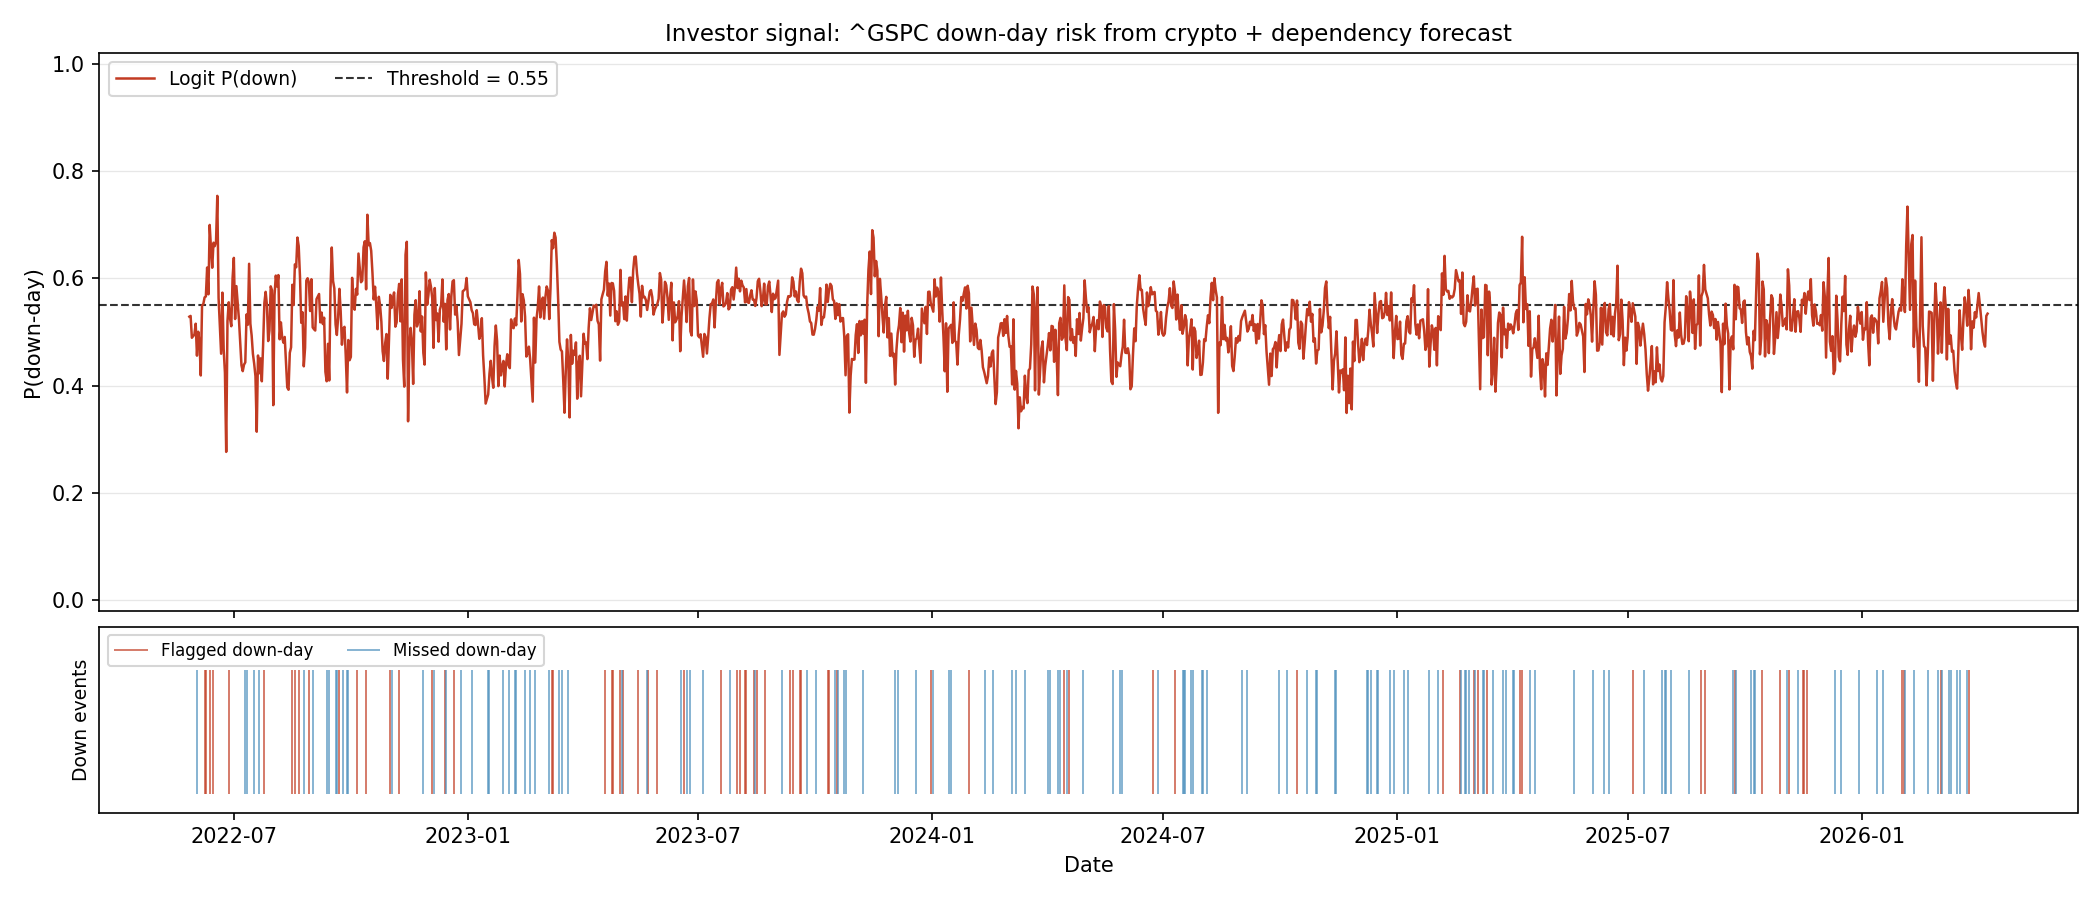
\includegraphics[width=0.9\textwidth]{../outputs/figures/signal_corr_BTC-USD_^GSPC_w14.png}
    \caption{Supplementary S\&P 500 warning signal at the 14-day window.}
    \label{fig:app_signal_gspc_w14}
\end{figure}

\begin{figure}[H]
    \centering
    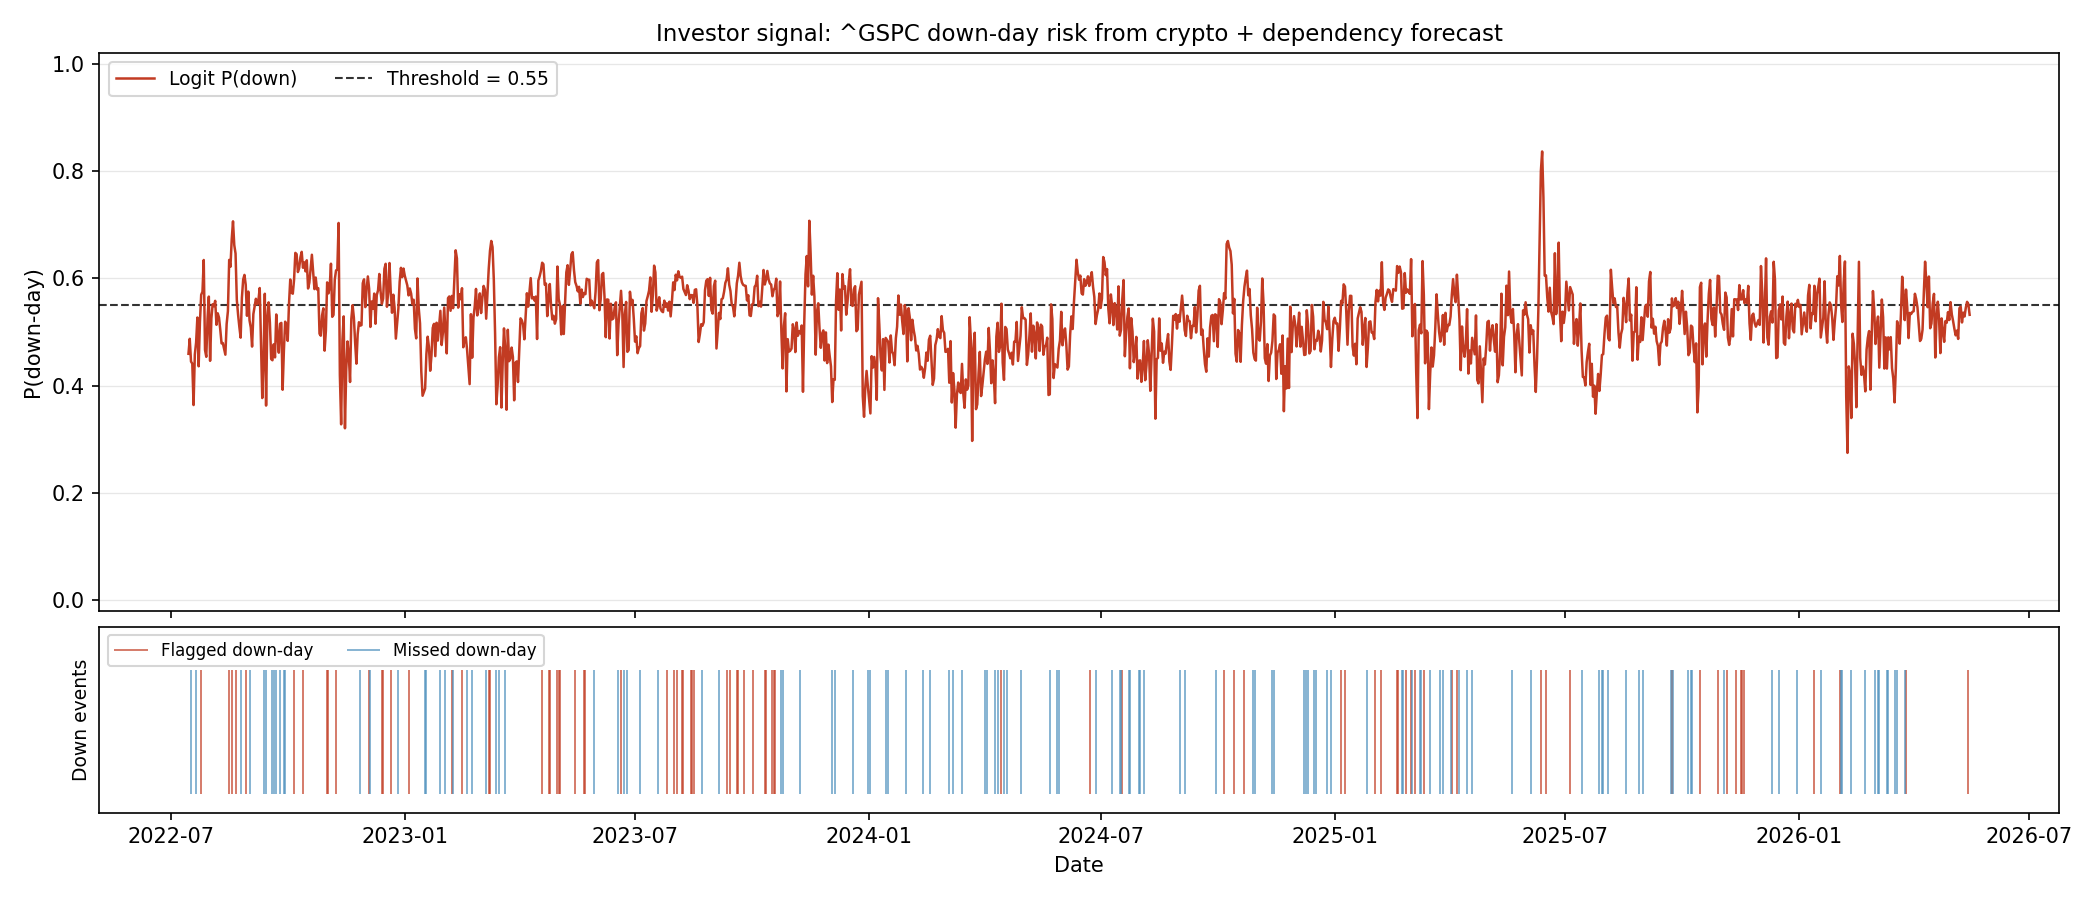
\includegraphics[width=0.9\textwidth]{../outputs/figures/signal_corr_BTC-USD_^GSPC_w60.png}
    \caption{Supplementary S\&P 500 warning signal at the 60-day window.}
    \label{fig:app_signal_gspc_w60}
\end{figure}

\begin{figure}[H]
    \centering
    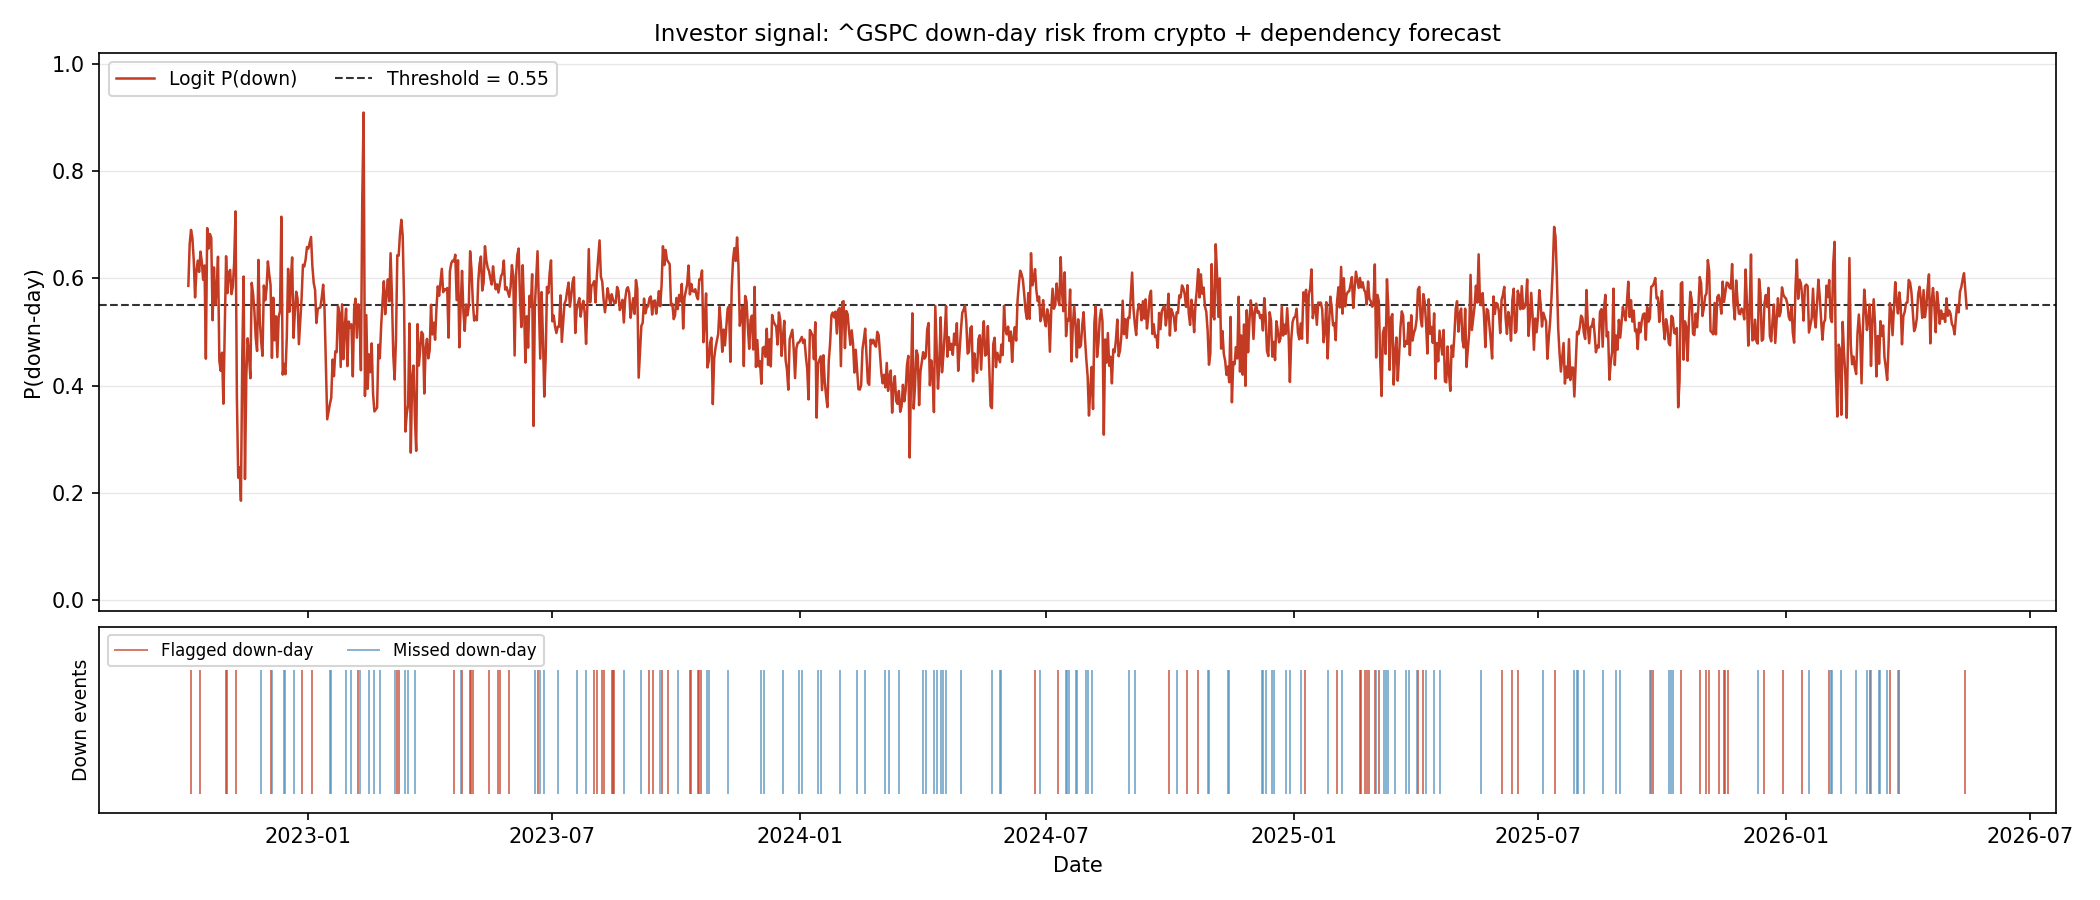
\includegraphics[width=0.9\textwidth]{../outputs/figures/signal_corr_BTC-USD_^GSPC_w90.png}
    \caption{Supplementary S\&P 500 warning signal at the 90-day window.}
    \label{fig:app_signal_gspc_w90}
\end{figure}

\begin{figure}[H]
    \centering
    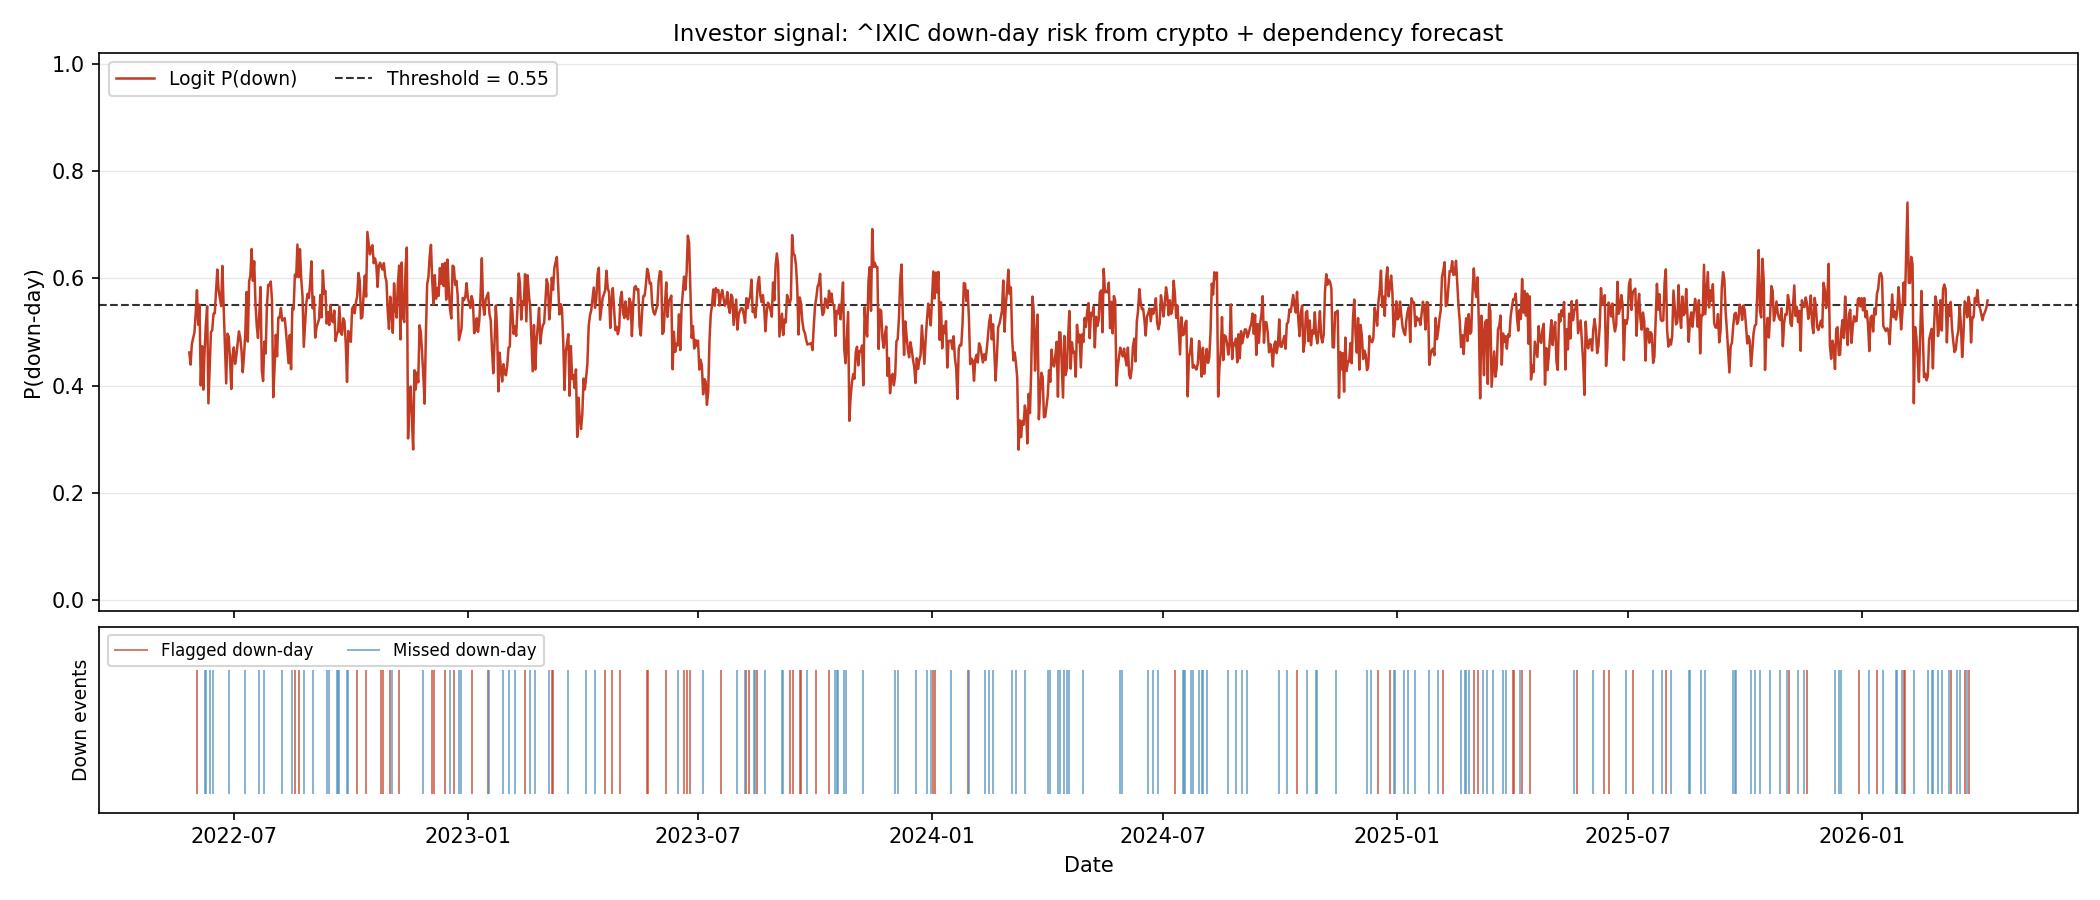
\includegraphics[width=0.9\textwidth]{../outputs/figures/signal_corr_BTC-USD_^IXIC_w14.png}
    \caption{Supplementary NASDAQ warning signal at the 14-day window.}
    \label{fig:app_signal_ixic_w14}
\end{figure}

\begin{figure}[H]
    \centering
    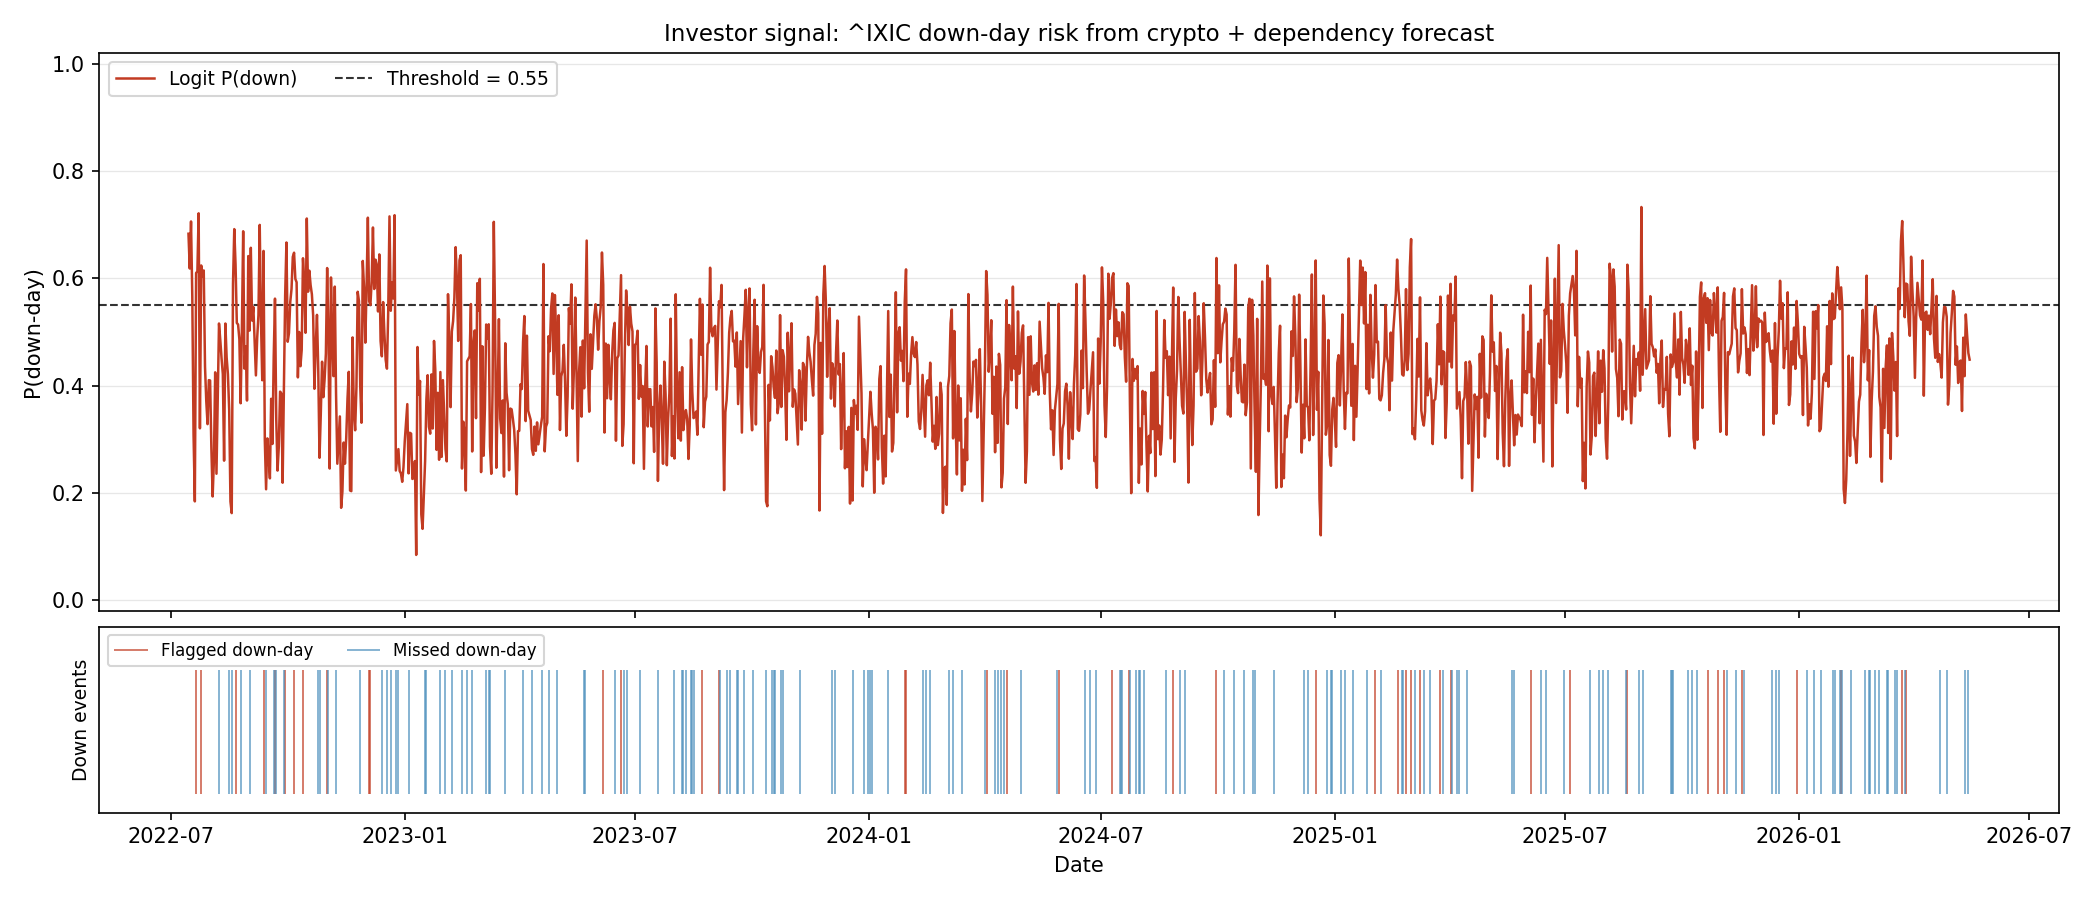
\includegraphics[width=0.9\textwidth]{../outputs/figures/signal_corr_BTC-USD_^IXIC_w60.png}
    \caption{Supplementary NASDAQ warning signal at the 60-day window.}
    \label{fig:app_signal_ixic_w60}
\end{figure}
